\section{Diagonalized mixed-hybrid method}
\def\mr{\mathring}
Model of flow described in section \ref{sc:darcy_flow} is solved by
mixed-hybrid formulation of finite elements method.
As in the previous chapter denote
$\tau$ time step and $\mathcal T_d$ regular simplex distribution of domain
$\Omega_d$, $d=1,2,3$.
Denote $\vc W_d(T_d)\subset \vc H(div,T_d)$
 space of Raviart-Thomas functions zero order ($RT_0$) on element $T_d\in 
\mathcal T_d$ and more
\[
    \vc W =  \vc W_1 \times \vc W_2 \times \vc W_3,\quad
    \vc W_d = \prod_{T_d\in \mathcal T_d} \vc W_d(T_d).
\]
Similarly introduce
\begin{equation}
Q=Q_{1}\times Q_{2}\times Q_{3},
\quad
Q_{d}=L^{2}\left(  \Omega_{d}\right).
\end{equation}
Then we introduce auxiliary space of values on element side $T_d\in \mathcal T_d$
\begin{equation}
    \mr Q(T_d)=\left\{  \mr q\in 
    L^{2}(\partial T_d \setminus  \partial\Omega_d^D):
    \mr q =\vc w\cdot \vc n|_{\partial T_d},
    \vc w\in\vc W_d%
    \right\}.
\end{equation}
and identify values on sides nonseparated by lower dimension element:
\begin{equation}
    \mr Q_d=\Big\{
        \mr q\in\prod_{T \in \mathcal T_d} \mr Q(T);
        \ \mr q|_{\partial T}=\mr q|_{\partial \tilde T}%
        \quad\text{na hraně }F=\partial T\cap\partial \tilde T
        \quad\text{ pokud }F\cap\Omega_{d-1}=\emptyset
    \Big\}.
\end{equation}
At the end we introduce $\mr Q = \mr Q_1 \times \mr Q_2 \times \mr Q_3$.

To resolve issue of unsteady Darcy's flow by clasic 
\emph{mixed-hybrid method} we are looking for trio $(\mathbf{u},h,\mr h)  
\in \vc W\times Q\times\mr Q$ which satisfies saddle-point set
\begin{align}
    a(\vc u,\vc v)  +b(\vc v, p) + \mr b(\vc v, \mr p)
        &=\langle g,\vc v \rangle, \qquad\forall \vc v\in \vc W,
        \label{eq:hybrid-frac-1}\\
    b(\vc u, q ) + \mr b( \vc u, \mr q) - c(p, \mr p, q, \mr q)
        &= \langle f, (q,\mr q) \rangle,
        \qquad\forall q\in Q,\ \mr q\in \mr Q, 
        \label{eq:hybrid-frac-2}
\end{align}
where
\begin{align}
    \label{eq:weak_term_a}
    a(\vc u, \vc v) &= \sum_{d=1}^{3}\sum_{T\in \mathcal T_d}
    \int_{T} \frac{1}{\delta_{d}}\tn K_{d}^{-1} 
    \vc u_d\cdot \vc v_d\,dx,
    \\
    \label{eq:weak_term_b}
    b(\vc u, q)  &= -\sum_{d=1}^{3}\sum_{T\in \mathcal T_d}
    \int_{T} q_d\,\div \vc u_d\,dx,
    \\
    \label{eq:weak_term_bf}
    \mr b(\vc u, \mr q)   &= \sum_{d=1}^{3}\sum_{T\in \mathcal T_d}
    \int_{\partial T\setminus\partial\Omega_{d}}
        \mr q|_{\partial T} ( \vc u_d\cdot\vc n)\,ds,
    \\
    \label{eq:weak_term c}
    c(h, \mr h, q, \mr q) &= c_f(h, \mr h, q, \mr q) 
    + c_t(h, \mr h, q, \mr q) + c_R(\mr h, \mr q)
    \\
    c_f(h, \mr h, q, \mr q)&=\sum_{d=2,3}\sum_{T\in \mathcal T_d}
        \int_{\partial T \cap\Omega_{d-1}} \sigma_{d} 
        (p_{d-1} - \mr p_d)(q_{d-1} - \mr q_d)\,ds
    \\
    c_t(h, \mr h, q, \mr q)&= \sum_{d=1}^{3}\sum_{T\in \mathcal T_d}
        \int_{T} \frac{\delta_d S_d}{\tau} h_d q_d\,dx,
    \\    
    c_R(\mr h, \mr q)&=
    \int_{\partial T\setminus\partial\Omega_{d}}
        \sigma_d^R\, h_d \mr q_d \,ds,
    \\
    \langle g, \vc v \rangle  & =
    -\sum_{d=1}^{3}\sum_{T\in\mathcal T_d}
    \int_{\partial T\cap\partial\Omega_N} 
        p_d^D\, (\vc v \cdot \vc n)  \,ds,
    \\
    \langle f, q \rangle  &=
    -\sum_{d=1}^{3}\int_{\Omega_d} \delta_{d}\,f_d\,q_{d}\,dx,
    \\
        &\phantom{=}+
    \sum_{d=1}^{3}\sum_{T\in\mathcal T_d}
    \int_{\partial T\cap\partial\Omega_N} 
        q_d^N \mr q_d - \sigma_d^R\, h_d^R \mr q_d\,ds
    \\
        &\phantom{=}-c_t(\tilde h, \mr{\tilde{h}}, q, \mr q).
    \label{eq:weak_term_f}%    
\end{align}
All quantities are meant in time $t$, only $\tilde h$ is pressure in time $t-\tau$.

The advantage of mixed-hybrid method is, the set of equations $(\ref{eq:hybrid-frac-1} - 
\ref{eq:hybrid-frac-2})$ can be reduced by eliminating variables $\vc u$ and $q$
to sparse positive definite set for variable $\mr q$.
This equation can then be efficiently solved using a~preconditioned conjugate gradient method.
Unfortunately, it appears that the resulting system does not satisfy the discrete maximum principle
 which in particular for short time steps $\tau$ can lead to unphysical oscillations.
One possible solution is diagonalization of method (lumped mixed-hybrid method)
 proposed in \cite{younes_2006}.
This method was implemented in Flow123d.
Consists in replacing the form $c_t$ by the form
\[
    c_t(h, \mr h, q, \mr q)= \sum_{d=1}^{3}\sum_{T\in \mathcal T_d}
        \sum_{i=1}^{d+1} \alpha_{T,i} \abs{T} \frac{\delta_d S_d}{\tau} 
        \left(\mr h|_{S_{T,i}}\,  \mr q|_{S_{T,i}}\right),
\]
where $\abs{T}$ is size of element, $S_{T,i}$ is side $i$ of element $T$, and 
$\mr h|_{S_{T,i}}$ is degreeof freedom on side whicj is identical with side $S_{T,i}$. 
Weights $\alpha_{T,i}$ can be chosen $1/d$. 
After solving the set of equations it is necessary to modify the velocity field $\vc u$
 adding the time term.
This modified the set of equations no longer meets the discrete maximum principle
 and shows oscillations.
Figure \ref{fig:LMH} is a comparison of the results
 use conventional MH scheme and LMH scheme.
At the MH scheme are noticeable oscillations wavefront
 and the minimum value is significantly less than zero.

\begin{figure}
    \begin{center}
       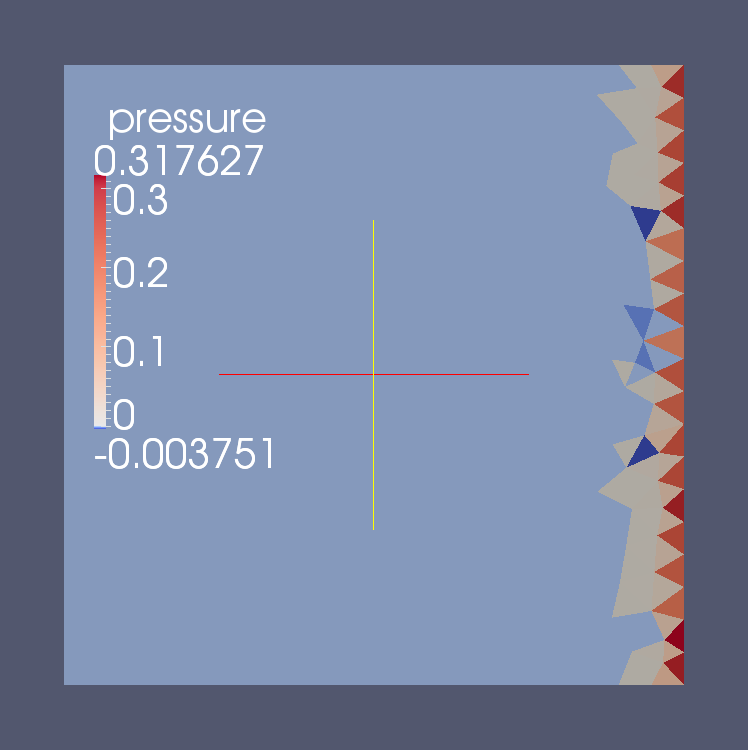
\includegraphics[width=0.4\textwidth]{figures/MH.png}
       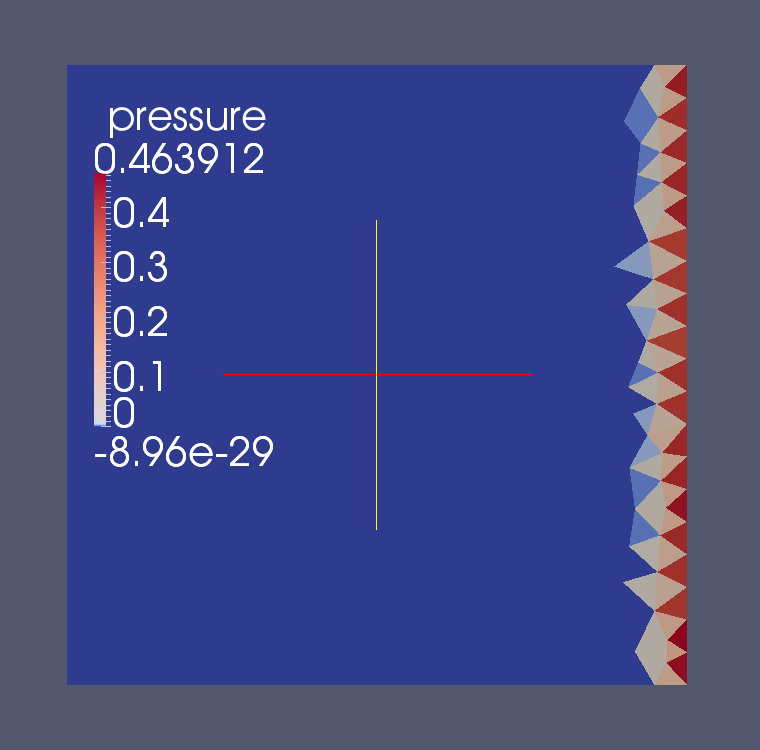
\includegraphics[width=0.405\textwidth]{figures/LMH.png}        
    \end{center}
    \caption{comparison of MH scheme (left) and LMH scheme (right), $\tau=10^{-4}$.}
    \label{fig:LMH}
\end{figure}

